% Created by tikzDevice version 0.7.0 on 2015-04-30 10:54:39
% !TEX encoding = UTF-8 Unicode
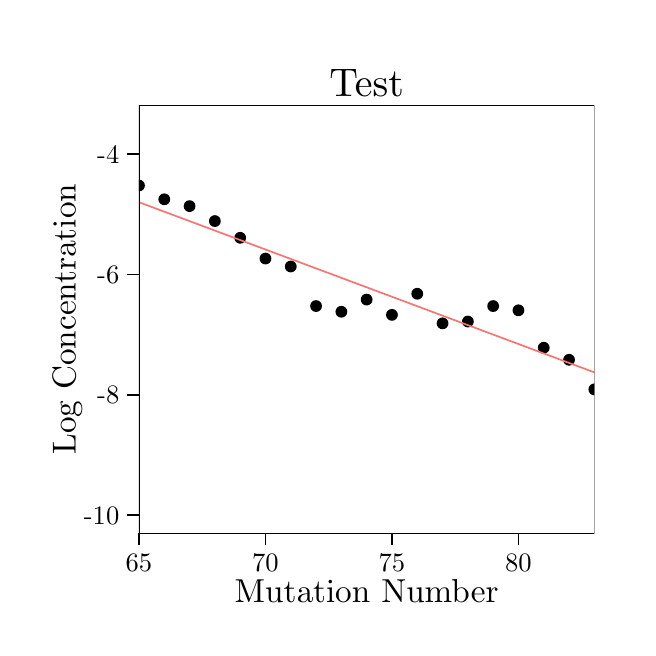
\begin{tikzpicture}[x=1pt,y=1pt]
\definecolor[named]{fillColor}{rgb}{1.00,1.00,1.00}
\path[use as bounding box,fill=fillColor,fill opacity=0.00] (0,0) rectangle (216.81,216.81);
\begin{scope}
\path[clip] (  0.00,  0.00) rectangle (216.81,216.81);
\definecolor[named]{drawColor}{rgb}{1.00,1.00,1.00}
\definecolor[named]{fillColor}{rgb}{1.00,1.00,1.00}

\path[draw=drawColor,line width= 0.6pt,line join=round,line cap=round,fill=fillColor] (  0.00,  0.00) rectangle (216.81,216.81);
\end{scope}
\begin{scope}
\path[clip] ( 40.22, 34.03) rectangle (204.76,188.82);
\definecolor[named]{fillColor}{rgb}{1.00,1.00,1.00}

\path[fill=fillColor] ( 40.22, 34.03) rectangle (204.76,188.82);
\definecolor[named]{fillColor}{rgb}{0.00,0.00,0.00}

\path[fill=fillColor] ( 40.22,159.77) circle (  2.13);

\path[fill=fillColor] ( 49.36,154.79) circle (  2.13);

\path[fill=fillColor] ( 58.50,152.32) circle (  2.13);

\path[fill=fillColor] ( 67.64,146.93) circle (  2.13);

\path[fill=fillColor] ( 76.79,140.88) circle (  2.13);

\path[fill=fillColor] ( 85.93,133.38) circle (  2.13);

\path[fill=fillColor] ( 95.07,130.51) circle (  2.13);

\path[fill=fillColor] (104.21,116.21) circle (  2.13);

\path[fill=fillColor] (113.35,114.15) circle (  2.13);

\path[fill=fillColor] (122.49,118.55) circle (  2.13);

\path[fill=fillColor] (131.63,113.03) circle (  2.13);

\path[fill=fillColor] (140.78,120.66) circle (  2.13);

\path[fill=fillColor] (149.92,109.97) circle (  2.13);

\path[fill=fillColor] (159.06,110.62) circle (  2.13);

\path[fill=fillColor] (168.20,116.21) circle (  2.13);

\path[fill=fillColor] (177.34,114.68) circle (  2.13);

\path[fill=fillColor] (186.48,101.16) circle (  2.13);

\path[fill=fillColor] (195.62, 96.80) circle (  2.13);

\path[fill=fillColor] (204.76, 86.11) circle (  2.13);
\definecolor[named]{drawColor}{rgb}{0.97,0.46,0.43}
\definecolor[named]{fillColor}{rgb}{0.97,0.46,0.43}

\path[draw=drawColor,line width= 0.6pt,line join=round,fill=fillColor] ( 40.22,153.73) -- (204.76, 92.25);
\definecolor[named]{drawColor}{rgb}{0.00,0.00,0.00}

\path[draw=drawColor,line width= 0.6pt,line join=round,line cap=round] ( 40.22, 34.03) rectangle (204.76,188.82);
\end{scope}
\begin{scope}
\path[clip] (  0.00,  0.00) rectangle (216.81,216.81);
\definecolor[named]{drawColor}{rgb}{0.00,0.00,0.00}

\node[text=drawColor,anchor=base east,inner sep=0pt, outer sep=0pt, scale=  0.96] at ( 33.11, 37.44) {-10};

\node[text=drawColor,anchor=base east,inner sep=0pt, outer sep=0pt, scale=  0.96] at ( 33.11, 80.87) {-8};

\node[text=drawColor,anchor=base east,inner sep=0pt, outer sep=0pt, scale=  0.96] at ( 33.11,124.31) {-6};

\node[text=drawColor,anchor=base east,inner sep=0pt, outer sep=0pt, scale=  0.96] at ( 33.11,167.74) {-4};
\end{scope}
\begin{scope}
\path[clip] (  0.00,  0.00) rectangle (216.81,216.81);
\definecolor[named]{drawColor}{rgb}{0.00,0.00,0.00}

\path[draw=drawColor,line width= 0.6pt,line join=round] ( 35.95, 40.74) --
	( 40.22, 40.74);

\path[draw=drawColor,line width= 0.6pt,line join=round] ( 35.95, 84.18) --
	( 40.22, 84.18);

\path[draw=drawColor,line width= 0.6pt,line join=round] ( 35.95,127.61) --
	( 40.22,127.61);

\path[draw=drawColor,line width= 0.6pt,line join=round] ( 35.95,171.04) --
	( 40.22,171.04);
\end{scope}
\begin{scope}
\path[clip] (  0.00,  0.00) rectangle (216.81,216.81);
\definecolor[named]{drawColor}{rgb}{0.00,0.00,0.00}

\path[draw=drawColor,line width= 0.6pt,line join=round] ( 40.22, 29.77) --
	( 40.22, 34.03);

\path[draw=drawColor,line width= 0.6pt,line join=round] ( 85.93, 29.77) --
	( 85.93, 34.03);

\path[draw=drawColor,line width= 0.6pt,line join=round] (131.63, 29.77) --
	(131.63, 34.03);

\path[draw=drawColor,line width= 0.6pt,line join=round] (177.34, 29.77) --
	(177.34, 34.03);
\end{scope}
\begin{scope}
\path[clip] (  0.00,  0.00) rectangle (216.81,216.81);
\definecolor[named]{drawColor}{rgb}{0.00,0.00,0.00}

\node[text=drawColor,anchor=base,inner sep=0pt, outer sep=0pt, scale=  0.96] at ( 40.22, 20.31) {65};

\node[text=drawColor,anchor=base,inner sep=0pt, outer sep=0pt, scale=  0.96] at ( 85.93, 20.31) {70};

\node[text=drawColor,anchor=base,inner sep=0pt, outer sep=0pt, scale=  0.96] at (131.63, 20.31) {75};

\node[text=drawColor,anchor=base,inner sep=0pt, outer sep=0pt, scale=  0.96] at (177.34, 20.31) {80};
\end{scope}
\begin{scope}
\path[clip] (  0.00,  0.00) rectangle (216.81,216.81);
\definecolor[named]{drawColor}{rgb}{0.00,0.00,0.00}

\node[text=drawColor,anchor=base,inner sep=0pt, outer sep=0pt, scale=  1.20] at (122.49,  9.03) {Mutation Number};
\end{scope}
\begin{scope}
\path[clip] (  0.00,  0.00) rectangle (216.81,216.81);
\definecolor[named]{drawColor}{rgb}{0.00,0.00,0.00}

\node[text=drawColor,rotate= 90.00,anchor=base,inner sep=0pt, outer sep=0pt, scale=  1.20] at ( 17.30,111.43) {Log Concentration};
\end{scope}
\begin{scope}
\path[clip] (  0.00,  0.00) rectangle (216.81,216.81);
\definecolor[named]{drawColor}{rgb}{0.00,0.00,0.00}

\node[text=drawColor,anchor=base,inner sep=0pt, outer sep=0pt, scale=  1.44] at (122.49,191.84) {Test};
\end{scope}
\end{tikzpicture}
